% chapter3.tex (Solution Formulation)

\chapter{Extensions to Guessing Numbers}
\label{ch:prob}

This chapter builds on the more important aspects of the literature review. The first section gives a number of possible areas of research that were rejected for various reasons, be they ones of complication, time constraints or otherwise. Definitions required for the next chapter are also explained here. Finally, a theorem is stated linking the fractional guessing game to fractional routing, as an analogue to the theorem linking the ordinary guessing game to network coding.

\section{Some Ideas}
\label{sect:ideas}

As with most new technologies, little of the topic of guessing numbers is refined into a widely accepted theory. If, as in Section~\ref{sect:routing}, network coding is to be viewed as Thomson's discovery of the electron and subsequent discoveries of other subatomic particles, then guessing numbers may be viewed as a move away from the Newton's corpuscular theory towards the concept of wave-particle duality; the combining of two separate existing notions to explain more complicated phenomena in the field. As such, there is much to investigate in order to find the most beneficial advancements. Some of these advancements, then, will lead to an academic impasse. The following are some propositions that were either of little value or proved to be too tricky or time-consuming.

\subsection{Topological Equivalence of Networks}

An interesting first concept was to investigate the \emph{degree} of a given network --- the degree of the polynomial required to give an optimal solution, and investigate the topological properties of networks with equal degree. However, as mentioned in Section~\ref{sect:lin_v_nonlin}, there are very few networks that have been shown to require non-linear codes for optimal solutions. Demonstrating topological equivalence would require a number of networks requiring quadratic (degree $2$) solutions, yet more requiring cubic solutions, and so on. Finding single networks with these properties seems to be an entire topic in itself. Given the lack of networks known to have these properties, this was considered infeasible.

\subsection{Bipartite Graphs}

\begin{figure}[ht]
     \centering
     \subfigure[Bipartite graph with an ordinary public channel]{
          \label{fig:public_channel}
          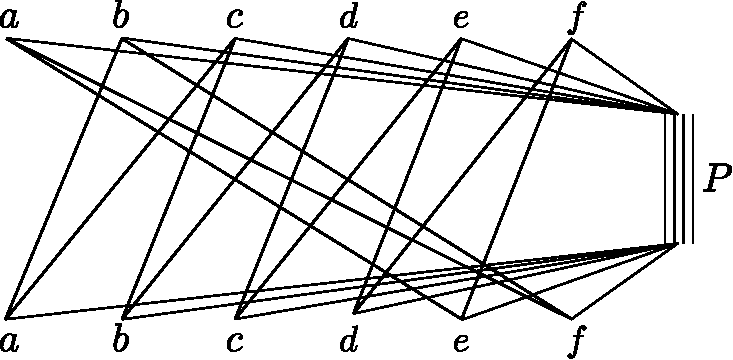
\includegraphics[width=.45\textwidth]{figures/public_channel.pdf}}
     \hspace{.3in}
     \subfigure[Bipartite graph with a second graph in place of the public channel]{
          \label{fig:public_channel_network}
          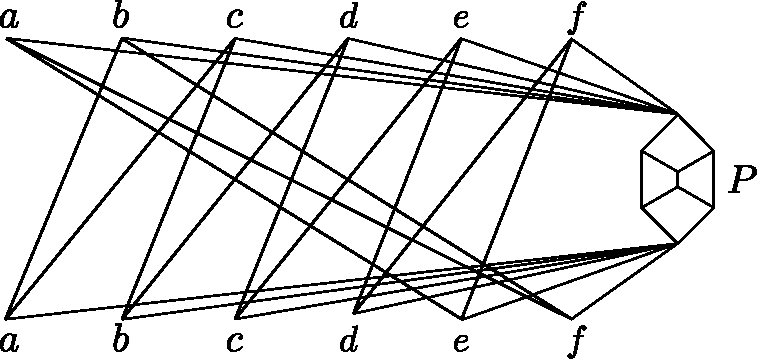
\includegraphics[width=.45\textwidth]{figures/public_channel_network.pdf}}

		 \caption[Public-channel problems with different types of channel]{Changing the ordinary public channel in \subref{fig:public_channel} to the more complicated version in \subref{fig:public_channel_network} does not help in finding a non-integer guessing number.}
\end{figure}

As mentioned in Section~\ref{sect:bipartite}, it is possible to change a guessing number problem into a public channel problem, by converting the graph into its bipartite representation and substituting a suitable public channel for the guessing part of the game --- if and only if the solution is linear \cite{riis2005util}. The intention was to generalise or expand the public-channel game so that it could also be used in the non-linear case, perhaps by replacing the public channel with another network (Figure~\ref{fig:public_channel_network}). However, this led to the circular problem in which a network with a non-integer guessing number was required to find a network with a non-integer guessing number.

If a public channel is added to a network with a non-linear solution, then the guessing number $k$ of that network may be increased, but the solution would then be an integer (i.e., a linear solution). It is not known, but would be interesting to investigate, whether the guessing number of the new graph would simply be $\lceil k \rceil$, the smallest integer not less than $k$.

\subsection{Delays and Error}

Many problems in network flow deal with delay-free (and error-free) networks, and indeed all problems concerning guessing numbers do not incorporate either delay or error-correcting codes. Real-world network flow problems may be translated into the theory of error-correcting codes \cite{riah2004}, but no work has yet been produced involving the graph-theory approach of guessing numbers.

The implications of introducing these real-world events on a guessing game is not immediately clear; however one may intuitively guess that any delay will improve the guessing number of a particular graph, and error will reduce it.

\section{Algebraic Calculations of Linear Guessing Numbers}

It is shown in \cite{riis2005util} that the \emph{linear guessing number} has an algebraic definition:

Let $M = (m_{ij})_{i, j}$ be an $n \times n \; (0, 1)$-matrix, and let $A$ be a finite field. Then define $\mathcal{C_A(M)}$ to be the class of $n \times n$ matrices $M^\prime = (m^\prime_{ij})_{i, j}$ with entries in the field $A$ for which $m_{ij} = 0 \Rightarrow m^\prime_{ij} = 0$. Let $I$ denote the $n \times n$ identity matrix and let $\mu(M) = n - \min_{M^\prime \in \mathcal{C_A(M)}} \mbox{rank}(I + M^\prime)$.

\begin{theorem}
 Let $G$ be a directed graph with $n$ nodes and adjacency matrix $M_G$. Let $A$ be a finite field. Then the graph $G$ has linear guessing number $k$ (over the field $A$) if and only if $\mu(G_N) = k$.
 \label{alg_gn}
\end{theorem}

\begin{remark}
 The reason that the identity matrix $I$ is added to the matrices $M^\prime$ is that the adjacency matrix $M$ (and therefore the matrices $M^\prime$) have zeroes along the diagonal. In practice, any element $a \in A$ could be consistently used along the diagonal, but each $a$ could be reduced to $1$ by adding linear combinations of other rows or columns.
\end{remark}

\subsection{Generalising Riis' Equations}

It is shown that it is possible to compute linear guessing numbers algebraically, by computing the ranks of a class of matrices. The linear guessing number has an algebraic definition $\mu(G_N)$ given above. It would be desirable if the algebraic definition could be extended to encompass non-linear guessing numbers. Network flow problems exist in the literature \cite{doug2005, riis2004} which only have non-linear solutions. Attempting to generalise the algebraic definition proves difficult, namely in finding the analogue of a `rank' in non-linear functions. Whilst one may use Gr\"obner bases to solve simultaneous polynomial equations, the notion of rank does not extend to allow computation of a non-linear guessing number. It is worth pointing out that it is possible to rewrite Theorem~\ref{alg_gn} for non-linear guessing numbers, but this would merely be restating their definition. Instead of the rank, some notion of ``whether this system is solvable'' would be used.

\section{Equivalence of Network Problems}

The process of reduction alters a network coding problem into exactly one problem in graph theory. The reverse, however, gives a class of networks. It can be shown that these network coding problems are equivalent, simply by considering the number of split moves and unsplit moves required to produce them (see Section~\ref{sect:guessing_number}).

If network $A$ and network $B$ are both produced from graph $G$, then $A$ and $B$ have the same source transmission bandwidth. If $A$ has global success rate $p$ then it is possible (and easy) to compute the global success rate of $B$ by first calculating the global success rate of $G$.

The motivation behind understanding this equivalence was to investigate if knowledge of it would allow investigation into the relationships between different network flow problems. However, it provided no extra information that was not already present in the literature; this equivalence would seem to be implicit, and as such is only made explicit here to clarify the link between network flow problems and their circuit representation.

\section{Extending the Guessing Game to Include Routing Capacity}
\label{sect:rgg}

An extension of the guessing game is to include the concept of routing capacity on the network. A co-operative game involving only routing capacity can be imagined by players only being allowed to concatenate the visible bits, without any other operations. The addition of network coding allows the players to perform arbitrary bit operations.

Transforming network coding problems into problems on graphs works by identifying source nodes with their respective sink nodes. The equivalent transformation in the routing capacity case results in asymmetrical, directed graphs.

\begin{figure}[ht]
	\centering
	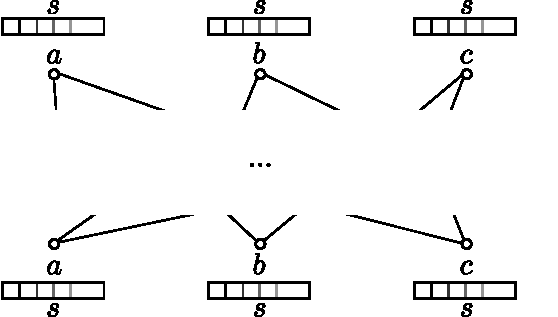
\includegraphics[width=250pt]{figures/asymm.pdf}
	\caption[Asymmetrical graph from a routing capacity problem]{Asymmetrical graph transformed from a problem in routing capacity. The internal nodes are arbitrary.}
	\label{asymm}
\end{figure}

The source nodes in Figure~\ref{asymm} are each transmitting messages of length $\log(s)$ bits. In general, the edges are of some capacity greater than $1$. This means that the (arbitrary) internal nodes must be able to handle concatenations of larger inputs for the receiver nodes to compute their required messages. Mathematically, however, it is more interesting to investigate symmetrical, undirected graphs.

It has been shown that the solutions over an alphabet $A$ (where $|A| = s$) of an information network flow problem $N \in \mathcal{C}_{mu}$ with $n$ input nodes and $n$ output nodes correspond directly with the optimal guessing strategies for a game played on $G_N$ over the same alphabet $A$, and that each strategy ensures that the players succeed with probability $s^{n - |G_N|}$ ($|G_N|$ being the number of vertices in $G_N$) \cite{riis2005util, riis2005info}.

The definition of the guessing game must be slightly modified to incorporate the different techniques used in routing problems as well as the size of the messages at the nodes. There is no longer a specific value $m_v \in A$, but a message consisting of bits from $A$.

The following is a formalisation of the new guessing game.

\begin{definition}

Let $\mathrm{RoutingGuessingGame}(G, s)$ or $\mathrm{RGG}(G, s)$ denote a co-operative game where each vertex $v \in V$ is assigned a message $m_v$. The message is actually a block $\mathbf{m_v} = m_1 m_2 m_3 \dots m_s$ where each $m_i \in A$. This message is then transmitted to each vertex $w$ with $(v, w) \in E$. In other words, vertex $w$ receives a set $M_w = \{m_v \in A^s : (v, w) \in E\}$. The goal is then to calculate the probability that the optimal protocol $\mathcal{P}$ (consisting of the functions $f_w : A^{s|M_w|} \rightarrow A^s$) succeeds.

\end{definition}

This definition is a minor modification of the ordinary guessing game where the alphabet $A$ is replaced with an alphabet $A^s$. The modification is motivated by the success of the specific guessing strategies highlighted in Chapter~\ref{ch:sol}, and allows us to capture the idea of fractional routing into the guessing game. As we will see, the game has a particularly nice solution if the size of the alphabet is a perfect square, where $s = t^2, t \in \NN, t > 1$. This corresponds to a version of the dice game where each player is assigned two dice values $x, y \in \{1, 2, \dots, t\}$ (see Section~\ref{sect:pentagon-proof}).

The definition above describes the messages as bit strings, but for the case where $s$ is a perfect square this is not really an appropriate definition since perfect squares are rarely a power of $2$. It is possible to write the strings in a different base to achieve the desired effect, but in fact it makes more sense to write the problem as an entropy argument. This is motivated by proofs which appear in Chapter~\ref{ch:sol}.

In this setting, the message $m_v$ should be viewed as a collection of independent variables $\mathcal{M}_v = \{ X_{v, 1}, X_{v, 2}, \dots, X_{v, s} \}$, where each $X_{v, r}$ are statistically independent, so the joint entropy is equal to the sum of the individual entropies: $H(A, B) = H(A) + H(B)$, for any $A, B \in \mathcal{M}_v$.

As mentioned in Section~\ref{sect:guessing_number}, a multiple-unicast network $N$ has a solution over an alphabet $A$ if and only if the corresponding graph $G_N$ has a guessing number not less than the number of input/output nodes in $N$. In exactly the same manner we can relate the new fractional guessing game defined above to fractional routing by the same theorem, the result of which is outlined below.

\begin{theorem}
A circuit information flow problem $N$ with $n$ input / output nodes has a fractional routing solution using words of length $k$ if and only if the guessing number of the corresponding graph $G_N$ has a fractional guessing number not less than $n$.
\end{theorem}

\section{Summary}

This chapter discusses various ideas for the progression of the thesis. Of the many ideas that were suggested, the more interesting research areas have been highlighted here, together with reasons for their infeasibility. Given time and other resources, it is entirely possible that such areas of work may produce fruitful work, hence their inclusion here.

In addition, a number of definitions are provided here as a precursor to Chapter~\ref{ch:sol}. The main definition given of the fractional guessing game, which combines fractional routing and guessing numbers. This modified game will be used in the next chapter, which will discuss applications of the new game in solving particular problems in graph theory and network flow.